\subsection{Model Formulations and Validation}
Simulations implemented ABAQUS (2017) software for quasi-static, implicit computations using user subroutines UMAT. Samples are modelled as continuous, homogeneous and isotropic elastic materials with Young's modulus and Poisson ratio comparable to biomolecules\cite{kurland2012measurement}. To eliminate the hourglass effect, R3D10 tetrahedral elements are employed\cite{hibbitt1984abaqus}.  Simulations impliment "surface to surface contact" interaction with "hard", nonadhesive normal contact and "rough" (Coulomb friction), non-slip tangential contact. 
% Boundary conditions fix the base of the structures, and vertical force and indentation data are mapped and sampled via reference points at the indenter's centre.

The shape of a blunt AFM tip, presented in Figure \ref{fig: ABAQUS Model-Setup}A, is a simplified construct similar to the SEM image of actual AFM tips shown by Chen \textit{et al.}\cite{chen_luo_doudevski_erten_kim_2019}. The tip is modelled as a rigid (incompressible) cone with opening angle $\theta = 20^o$ ending in a spherical termination of radius $R$\cite{canet2014correction}. The spherical portion smoothly transitions to the conical segment at the tangential contact point described by,

\begin{equation}\label{eq: AFM Tip}
\begin{split}
    X_{tangent} = R\cos\theta 
    \\
    Y_{tangent} = R(1-\sin\theta) 
\end{split}
\end{equation}

Therefore, the tip can be considered spherical for indentations $\delta/R < 1-\sin(\theta) \approx 0.65$, which allows for a direct comparison with analytical indentation models. These theoretical indentation models characterise the behaviour of the simulated indentation. The Hertz model describes contact between a sphere and an elastic half-space, defining the indentation force, $F$\cite{hertz1881contact,hertz1882contact,hertz1896contact},

\begin{equation} F_{Hertz}(\delta_{12}) =  \frac{4}{3} \frac{E}{(1-\nu^2)} \sqrt{R^*} \delta_{12}^{3/2} \label{eq: Hertz} \end{equation}

for indentation depth $\delta_{12}$, Young’s modulus $E$, Poisson’s ratio $\nu$, and tip-surface contact radius $R^*$. Where $\frac{1}{R^*} = \frac{1}{R} + \frac{1}{r}$, with indenter radius $R$ and surface radius $r$. Applying the Hertzian analysis to conical indenters, we recover the Sneddon model\cite{sneddon1965relation}. For spherical samples, a modified Sneddon model developed by Han \textit{et al.}\cite{han2021modified} is given as,

\begin{equation}F_{Sneddon}(\delta_{12}) = \frac{2}{\pi}\frac{E}{(1-\nu^2)} \cdot tan(\theta)\delta^{2} \cdot f\left(\frac{\delta}{2r}\right)\label{eq: Sneddon}\end{equation}

\begin{equation}  f\left(\frac{\delta}{2r}\right) = 1+ \gamma \left(\frac{\delta}{2r}\right) \end{equation}

\begin{equation} \gamma = -5.103\nu^2 - 13.99\nu + 13.53 \end{equation}

where $\theta$ is the indenters principle angle. However, as shown by Glaubitz \textit{et al.}\cite{glaubitz2014novel}, compression of soft spherical samples during indentation leads to significant underestimations of Young's modulus when analysing the AFM force curves with the simple Hertz model. "Double Contact" models\cite{glaubitz2014novel, dokukin2013quantitative} account for compression produced by spherical indenters as such,

\begin{equation}  F_{Double}(\delta_{12}) =  \frac{4}{3} \frac{E}{(1-\nu^2)} \left[ \frac{(R^*r)^{1/3}}{R^{* 1/3}+r^{1/3}} \right]^{3/2}\delta_{12}^{3/2} \label{eq: Hertz Double Contact}\end{equation}

Applying ABAQUS to AFM indentation into elastic spheres of varying radii provides a robust validation of simulation accuracy through comparison with the theoretical contact models. Following the common experimental determination of Young modulus\cite{sun2021determination,DIMITRIADIS20022798, vinckier1998measuring, kontomaris2019determination, kontomaris2020hertz}, theoretical contact models are used to fit the Young modulus for simulated indentation force curves of elastic spheres. The elastic sphere moves freely with a fixed, rigid base beneath. Restricting indentation to the z-axis allows the modelling to be asymmetrically centred around the z-axis.

\begin{figure}[ht]
    \centering
    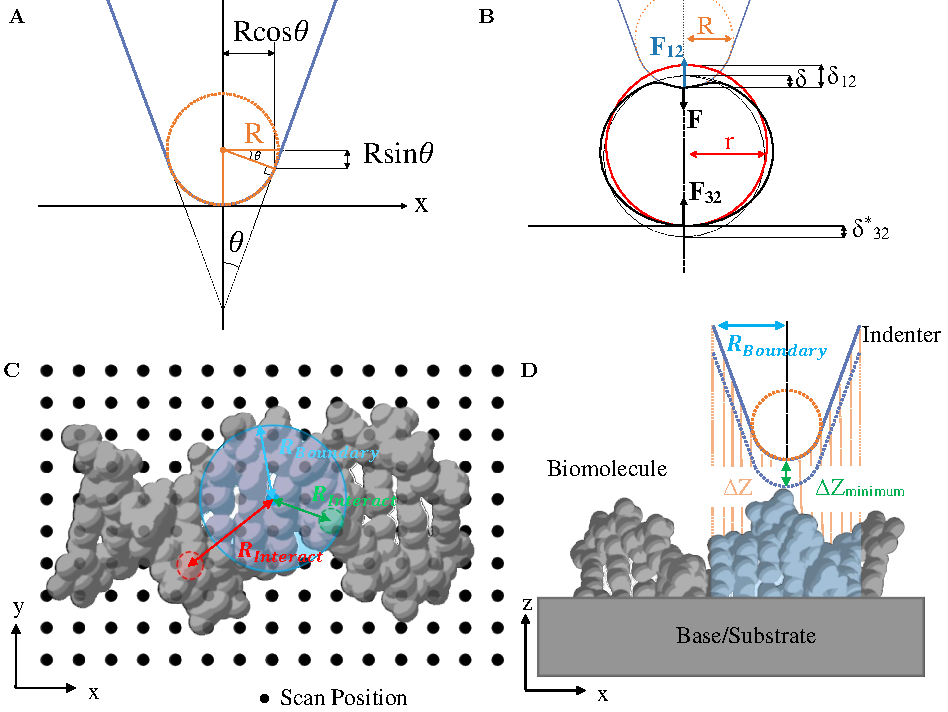
\includegraphics[width=1\linewidth]{Figures/Figure1.pdf}    
    \caption{\label{fig: ABAQUS Model-Setup} (A) Illustration of AFM tip geometry as a rigid cone with opening angle $\theta$ ending in a spherical termination of radius $R$. (B) ABAQUS model assembly from elastic indentation tests. Modelled asymmetrically using elastic spheres modelled as semi-circles with a rigid base beneath. (C-D)Schematic diagrams illustrating the calculation of initial scan heights in AFM code. (C) Illustration of the calculation atoms on the surface within the indenters boundary. Black dots represent the XY grid of scan positions. The calculation is restricted to the XY plane in which only atoms inside the radial extent of the indenters, $R_{Boundary}$ (blue), are calculated. The red atom represents an atom outside the extent and thus is omitted, as appose to the green atom, which is included. (D) Illustration of calculation of heights for each given position. An array of all distances ($\Delta Z$) between the indenters and molecules surfaces are calculated (red). The minima of these distances thus give the translation distance to place the indenter in tangential contact.} 
\end{figure}